% =========================================================
\section{Results and Discussion}
\label{sec:results}

\subsection{Interface}

\begin{figure}[h!]
    \centering
    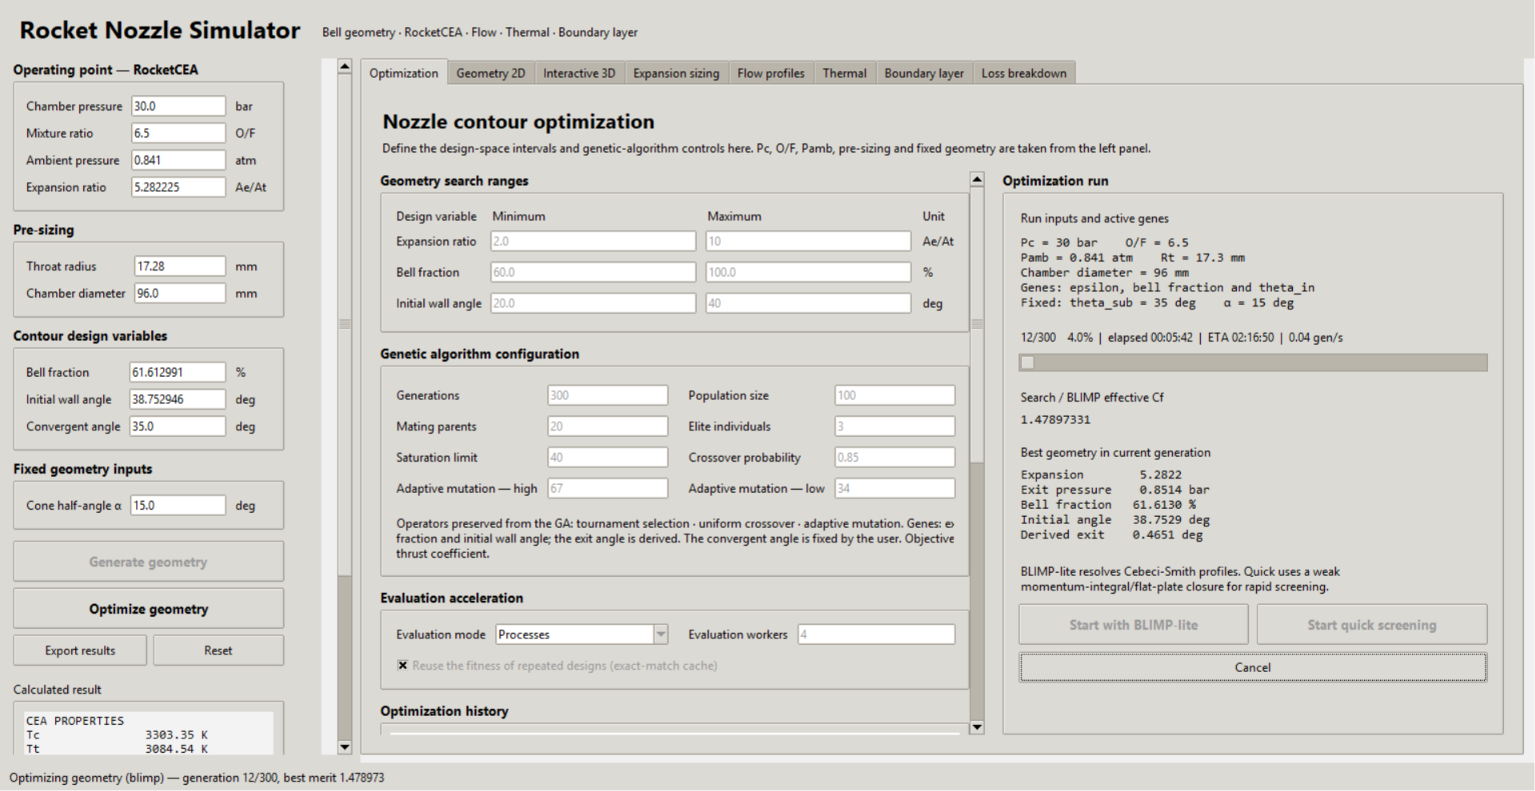
\includegraphics[width=1\linewidth]{int.png}
    \caption{Enter Caption}
    \label{fig:placeholder}
\end{figure}
% =========================================================

\subsection{Evaluation case and data provenance}

The following results use two complete simulator exports retained with the software.
Both cases use the same operating point and are evaluated with the BLIMP-lite closure,
so the comparison changes only the three optimized design variables. The manually
selected baseline is
\begin{equation}
\bm q_0=[5.6,\,0.80,\,30^\circ]^T,
\end{equation}
whereas the best geometry retained from an illustrative GA run is
\begin{equation}
\bm q^*=[5.071819,\,0.600180,\,39.30912^\circ]^T.
\end{equation}
The latter run used a
user-adjusted \(40^\circ\) upper bound for \(\theta_{in}\), rather than the current
\(35^\circ\) default.

\begin{table}[H]
\centering
\caption{Fixed operating-point and pre-sizing inputs used in the comparison.}
\label{tab:result_fixed_inputs}
\begin{tabular}{lll}
\toprule
Quantity & Symbol & Value \\
\midrule
Chamber pressure & \(p_c\) & \(30\,\mathrm{bar}\) \\
Mixture ratio & \(O/F\) & 6.5 \\
Ambient pressure & \(p_a\) & \(0.841\,\mathrm{atm}\) \\
Throat radius & \(r_t\) & \(17.28\,\mathrm{mm}\) \\
Chamber diameter & \(D_c\) & \(120\,\mathrm{mm}\) \\
Convergent angle & \(\theta_{sub}\) & \(50^\circ\) \\
Reference cone half-angle & \(\alpha\) & \(15^\circ\) \\
\bottomrule
\end{tabular}
\end{table}

The CSV files used by the plots below are included with the manuscript. Consequently,
the figures are generated by PGFPlots from the numerical exports rather than inserted
as screenshots. Since the saved run did not retain a random seed or complete population
history, it is reported as a representative optimization result, not as evidence of
statistical GA repeatability or guaranteed global optimality.

\subsection{Geometry selected by the loss-corrected objective}

\begin{table}[H]
\centering
\caption{Baseline and retained GA geometry.}
\label{tab:geometry_comparison}
\begin{tabular}{lrr}
\toprule
Quantity & Baseline & Retained GA candidate \\
\midrule
Expansion ratio, \(\varepsilon\) & 5.6000 & 5.0718 \\
Bell fraction, \(K_b\) & 0.8000 & 0.6002 \\
Initial angle, \(\theta_{in}\) & \(30.000^\circ\) & \(39.309^\circ\) \\
Derived exit angle, \(\theta_{out}\) & \(3.790^\circ\) & \(0.550^\circ\) \\
Total axial length & \(121.886\,\mathrm{mm}\) & \(100.774\,\mathrm{mm}\) \\
\bottomrule
\end{tabular}
\end{table}

\begin{figure}[H]
\centering
\begin{tikzpicture}
\begin{axis}[
    width=0.94\linewidth,
    height=0.48\linewidth,
    xlabel={Axial position [mm]},
    ylabel={Radius [mm]},
    grid=both,
    xmin=0,
    xmax=128,
    ymin=-65,
    ymax=65,
    legend style={at={(0.98,0.98)},anchor=north east,fill=white},
]
\addplot[blue,thick] table[x=x_mm,y=radius_mm,col sep=comma]
    {Images/baseline_geometry.csv};
\addplot[blue,thick,forget plot] table[x=x_mm,y expr=-\thisrow{radius_mm},col sep=comma]
    {Images/baseline_geometry.csv};
\addplot[red!75!black,thick,dashed] table[x=x_mm,y=radius_mm,col sep=comma]
    {Images/optimized_geometry.csv};
\addplot[red!75!black,thick,dashed,forget plot]
    table[x=x_mm,y expr=-\thisrow{radius_mm},col sep=comma]
    {Images/optimized_geometry.csv};
\legend{Baseline,Retained GA candidate}
\end{axis}
\end{tikzpicture}
\caption{Baseline and retained GA contours generated directly from the exported coordinates.}
\label{fig:optimized_geometry_comparison}
\end{figure}

The selected geometry is \(17.32\%\) shorter in total axial length. The higher
initial angle creates stronger early expansion, while the quadratic closure reduces
the derived exit angle to approximately \(0.55^\circ\). This result must be read
together with the model limitations: there is no independent MOC or shock-structure
analysis penalizing rapid internal turning. The admissible bounds therefore remain an
important part of the engineering definition of the search space.

\subsection{Effective thrust coefficient and loss decomposition}

\begin{table}[H]
\centering
\caption{BLIMP-lite performance comparison at the specified ambient pressure.}
\label{tab:performance_comparison}
\begin{tabular}{lrr}
\toprule
Quantity & Baseline & Retained GA candidate \\
\midrule
Exit pressure, \(p_e\) [bar] & 0.7834 & 0.9024 \\
Exit condition & Overexpanded & Underexpanded \\
\(C_{F,mom}^{CEA}\) & 1.511664 & 1.490527 \\
\(\eta_{div}\) & 0.998906 & 0.999977 \\
\(\eta_{BL}\) & 0.996066 & 0.996610 \\
\(C_{F,p}\) & -0.012839 & 0.008504 \\
\(C_{F,fric}\) & 0.017646 & 0.014309 \\
\(C_{F,eff}\) & 1.473586 & 1.479634 \\
Effective thrust [N] & 4147.0 & 4164.0 \\
\bottomrule
\end{tabular}
\end{table}

\begin{figure}[H]
\centering
\begin{tikzpicture}
\begin{axis}[
    ybar,
    bar width=9pt,
    width=0.94\linewidth,
    height=0.50\linewidth,
    ylabel={Modelled decrement, $\Delta C_F$},
    symbolic x coords={Divergence,BL_blockage,Wall_friction,Ambient_mismatch},
    xtick=data,
    xticklabels={Divergence,BL blockage,Wall friction,Ambient mismatch},
    x tick label style={rotate=18,anchor=east},
    ymin=0,
    grid=major,
    legend style={at={(0.5,1.03)},anchor=south,legend columns=2},
]
\addplot[fill=blue!55] table[x=mechanism,y=baseline,col sep=comma]
    {Images/loss_breakdown.csv};
\addplot[fill=red!60] table[x=mechanism,y=optimized,col sep=comma]
    {Images/loss_breakdown.csv};
\legend{Baseline,Retained GA candidate}
\end{axis}
\end{tikzpicture}
\caption{Non-negative loss contributions in thrust-coefficient units. A positive
pressure-thrust contribution is a gain and is therefore excluded from the ambient
mismatch bar.}
\label{fig:loss_breakdown_comparison}
\end{figure}

The effective thrust coefficient increases from 1.473586 to 1.479634, a \(0.41\%\)
improvement for fixed \(p_cA_t\). The retained candidate does not simply choose the
ideal pressure-matched expansion ratio \(\varepsilon_{ideal}=5.2792\). Instead, it
accepts a small positive pressure-thrust contribution and reduces the modelled wall
friction through the shorter contour. In the selected candidate, wall friction
accounts for approximately \(73.8\%\) of the non-negative modelled loss, boundary-layer
blockage for \(26.1\%\), and exit divergence for less than \(0.2\%\). These percentages
describe the implemented closure and must not be interpreted as experimentally
validated loss attribution.

\subsection{Axial flow and boundary-layer response}

\begin{figure}[H]
\centering
\begin{tikzpicture}
\begin{axis}[
    width=0.94\linewidth,
    height=0.46\linewidth,
    xlabel={Axial position [mm]},
    ylabel={Mach number},
    grid=both,
    legend pos=north west,
]
\addplot[blue,thick] table[x expr=1000*\thisrow{x_m},y=mach,col sep=comma]
    {Images/baseline_flow_profile.csv};
\addplot[red!75!black,thick,dashed]
    table[x expr=1000*\thisrow{x_m},y=mach,col sep=comma]
    {Images/optimized_flow_profile.csv};
\legend{Baseline,Retained GA candidate}
\end{axis}
\end{tikzpicture}
\caption{Quasi-one-dimensional Mach reconstruction for the two geometries.}
\label{fig:mach_comparison}
\end{figure}

\begin{figure}[H]
\centering
\begin{tikzpicture}
\begin{axis}[
    width=0.94\linewidth,
    height=0.46\linewidth,
    xlabel={Axial position [mm]},
    ylabel={Displacement thickness [mm]},
    grid=both,
    legend pos=north west,
]
\addplot[blue,thick]
    table[x expr=1000*\thisrow{x_m},y expr=1000*\thisrow{delta_star_m},col sep=comma]
    {Images/baseline_boundary_layer.csv};
\addplot[red!75!black,thick,dashed]
    table[x expr=1000*\thisrow{x_m},y expr=1000*\thisrow{delta_star_m},col sep=comma]
    {Images/optimized_boundary_layer.csv};
\legend{Baseline,Retained GA candidate}
\end{axis}
\end{tikzpicture}
\caption{BLIMP-lite compressible displacement-thickness distributions.}
\label{fig:displacement_thickness_comparison}
\end{figure}

The exported profiles remain finite and continuous across all four geometric
segments. The comparison also illustrates why \(\eta_{BL}\) and \(C_{F,fric}\) are
kept separate: the former represents the effective-area velocity correction, whereas
the latter is obtained by integrating the resolved wall shear. A publication-level
assessment of optimizer robustness will additionally require repeated seeded runs,
population convergence statistics and validation of the retained candidate with an
independent higher-fidelity method.
